% Created by tikzDevice version 0.12 on 2019-02-27 23:06:35
% !TEX encoding = UTF-8 Unicode
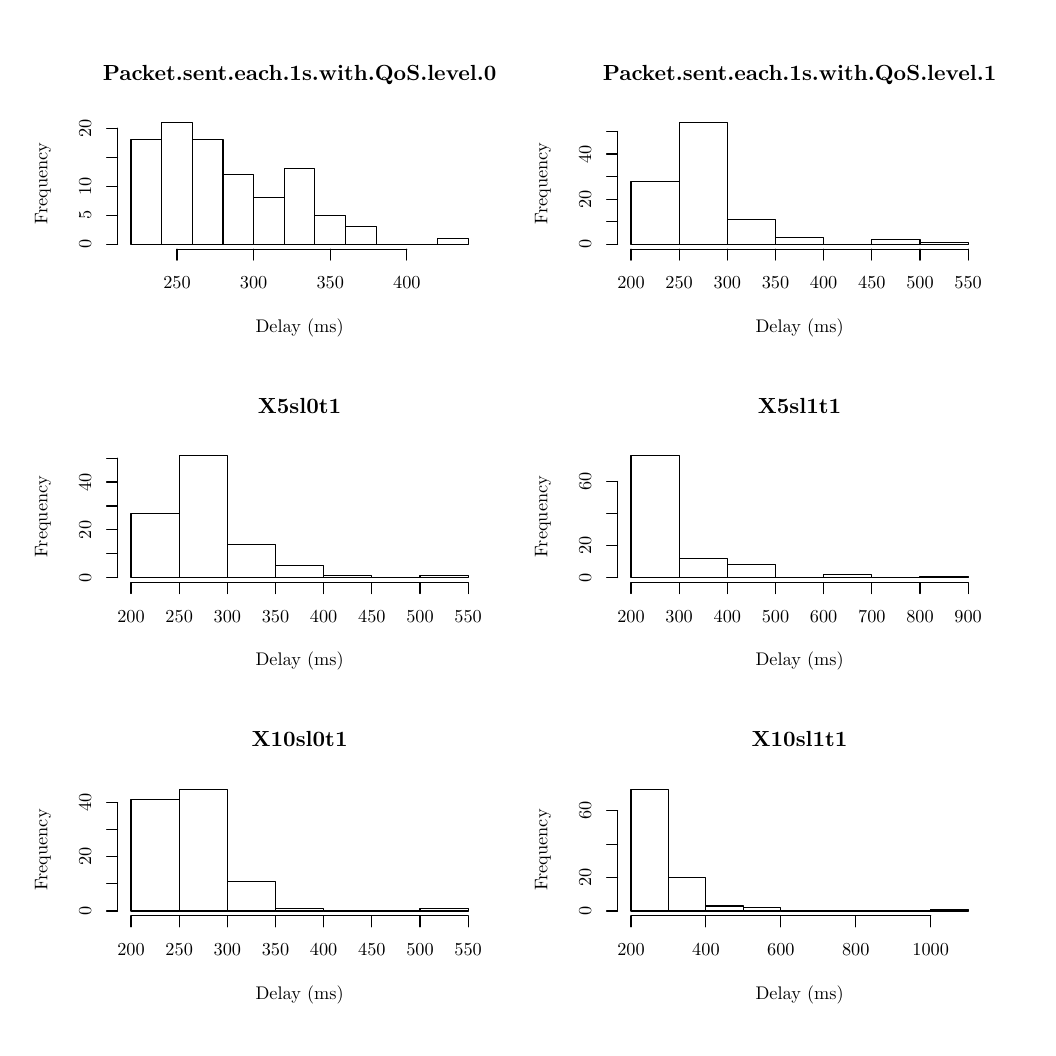
\begin{tikzpicture}[x=1pt,y=1pt]
\definecolor{fillColor}{RGB}{255,255,255}
\path[use as bounding box,fill=fillColor,fill opacity=0.00] (0,0) rectangle (361.35,361.35);
\begin{scope}
\path[clip] (  0.00,240.90) rectangle (180.67,361.35);
\definecolor{drawColor}{RGB}{0,0,0}

\node[text=drawColor,anchor=base,inner sep=0pt, outer sep=0pt, scale=  0.79] at ( 98.26,342.38) {\bfseries Packet.sent.each.1s.with.QoS.level.0};

\node[text=drawColor,anchor=base,inner sep=0pt, outer sep=0pt, scale=  0.66] at ( 98.26,251.20) {Delay (ms)};

\node[text=drawColor,rotate= 90.00,anchor=base,inner sep=0pt, outer sep=0pt, scale=  0.66] at (  7.13,305.08) {Frequency};
\end{scope}
\begin{scope}
\path[clip] (  0.00,  0.00) rectangle (361.35,361.35);
\definecolor{drawColor}{RGB}{0,0,0}

\path[draw=drawColor,line width= 0.4pt,line join=round,line cap=round] ( 53.96,281.29) -- (137.02,281.29);

\path[draw=drawColor,line width= 0.4pt,line join=round,line cap=round] ( 53.96,281.29) -- ( 53.96,277.33);

\path[draw=drawColor,line width= 0.4pt,line join=round,line cap=round] ( 81.64,281.29) -- ( 81.64,277.33);

\path[draw=drawColor,line width= 0.4pt,line join=round,line cap=round] (109.33,281.29) -- (109.33,277.33);

\path[draw=drawColor,line width= 0.4pt,line join=round,line cap=round] (137.02,281.29) -- (137.02,277.33);

\node[text=drawColor,anchor=base,inner sep=0pt, outer sep=0pt, scale=  0.66] at ( 53.96,267.04) {250};

\node[text=drawColor,anchor=base,inner sep=0pt, outer sep=0pt, scale=  0.66] at ( 81.64,267.04) {300};

\node[text=drawColor,anchor=base,inner sep=0pt, outer sep=0pt, scale=  0.66] at (109.33,267.04) {350};

\node[text=drawColor,anchor=base,inner sep=0pt, outer sep=0pt, scale=  0.66] at (137.02,267.04) {400};

\path[draw=drawColor,line width= 0.4pt,line join=round,line cap=round] ( 32.47,283.05) -- ( 32.47,325.02);

\path[draw=drawColor,line width= 0.4pt,line join=round,line cap=round] ( 32.47,283.05) -- ( 28.51,283.05);

\path[draw=drawColor,line width= 0.4pt,line join=round,line cap=round] ( 32.47,293.55) -- ( 28.51,293.55);

\path[draw=drawColor,line width= 0.4pt,line join=round,line cap=round] ( 32.47,304.04) -- ( 28.51,304.04);

\path[draw=drawColor,line width= 0.4pt,line join=round,line cap=round] ( 32.47,314.53) -- ( 28.51,314.53);

\path[draw=drawColor,line width= 0.4pt,line join=round,line cap=round] ( 32.47,325.02) -- ( 28.51,325.02);

\node[text=drawColor,rotate= 90.00,anchor=base,inner sep=0pt, outer sep=0pt, scale=  0.66] at ( 22.97,283.05) {0};

\node[text=drawColor,rotate= 90.00,anchor=base,inner sep=0pt, outer sep=0pt, scale=  0.66] at ( 22.97,293.55) {5};

\node[text=drawColor,rotate= 90.00,anchor=base,inner sep=0pt, outer sep=0pt, scale=  0.66] at ( 22.97,304.04) {10};

\node[text=drawColor,rotate= 90.00,anchor=base,inner sep=0pt, outer sep=0pt, scale=  0.66] at ( 22.97,325.02) {20};
\end{scope}
\begin{scope}
\path[clip] ( 32.47,281.29) rectangle (164.04,328.88);
\definecolor{drawColor}{RGB}{0,0,0}

\path[draw=drawColor,line width= 0.4pt,line join=round,line cap=round] ( 37.35,283.05) rectangle ( 48.42,320.82);

\path[draw=drawColor,line width= 0.4pt,line join=round,line cap=round] ( 48.42,283.05) rectangle ( 59.49,327.12);

\path[draw=drawColor,line width= 0.4pt,line join=round,line cap=round] ( 59.49,283.05) rectangle ( 70.57,320.82);

\path[draw=drawColor,line width= 0.4pt,line join=round,line cap=round] ( 70.57,283.05) rectangle ( 81.64,308.23);

\path[draw=drawColor,line width= 0.4pt,line join=round,line cap=round] ( 81.64,283.05) rectangle ( 92.72,299.84);

\path[draw=drawColor,line width= 0.4pt,line join=round,line cap=round] ( 92.72,283.05) rectangle (103.79,310.33);

\path[draw=drawColor,line width= 0.4pt,line join=round,line cap=round] (103.79,283.05) rectangle (114.87,293.55);

\path[draw=drawColor,line width= 0.4pt,line join=round,line cap=round] (114.87,283.05) rectangle (125.94,289.35);

\path[draw=drawColor,line width= 0.4pt,line join=round,line cap=round] (125.94,283.05) rectangle (137.02,283.05);

\path[draw=drawColor,line width= 0.4pt,line join=round,line cap=round] (137.02,283.05) rectangle (148.09,283.05);

\path[draw=drawColor,line width= 0.4pt,line join=round,line cap=round] (148.09,283.05) rectangle (159.17,285.15);
\end{scope}
\begin{scope}
\path[clip] (180.67,240.90) rectangle (361.35,361.35);
\definecolor{drawColor}{RGB}{0,0,0}

\node[text=drawColor,anchor=base,inner sep=0pt, outer sep=0pt, scale=  0.79] at (278.93,342.38) {\bfseries Packet.sent.each.1s.with.QoS.level.1};

\node[text=drawColor,anchor=base,inner sep=0pt, outer sep=0pt, scale=  0.66] at (278.93,251.20) {Delay (ms)};

\node[text=drawColor,rotate= 90.00,anchor=base,inner sep=0pt, outer sep=0pt, scale=  0.66] at (187.80,305.08) {Frequency};
\end{scope}
\begin{scope}
\path[clip] (  0.00,  0.00) rectangle (361.35,361.35);
\definecolor{drawColor}{RGB}{0,0,0}

\path[draw=drawColor,line width= 0.4pt,line join=round,line cap=round] (218.02,281.29) -- (339.84,281.29);

\path[draw=drawColor,line width= 0.4pt,line join=round,line cap=round] (218.02,281.29) -- (218.02,277.33);

\path[draw=drawColor,line width= 0.4pt,line join=round,line cap=round] (235.42,281.29) -- (235.42,277.33);

\path[draw=drawColor,line width= 0.4pt,line join=round,line cap=round] (252.83,281.29) -- (252.83,277.33);

\path[draw=drawColor,line width= 0.4pt,line join=round,line cap=round] (270.23,281.29) -- (270.23,277.33);

\path[draw=drawColor,line width= 0.4pt,line join=round,line cap=round] (287.63,281.29) -- (287.63,277.33);

\path[draw=drawColor,line width= 0.4pt,line join=round,line cap=round] (305.04,281.29) -- (305.04,277.33);

\path[draw=drawColor,line width= 0.4pt,line join=round,line cap=round] (322.44,281.29) -- (322.44,277.33);

\path[draw=drawColor,line width= 0.4pt,line join=round,line cap=round] (339.84,281.29) -- (339.84,277.33);

\node[text=drawColor,anchor=base,inner sep=0pt, outer sep=0pt, scale=  0.66] at (218.02,267.04) {200};

\node[text=drawColor,anchor=base,inner sep=0pt, outer sep=0pt, scale=  0.66] at (235.42,267.04) {250};

\node[text=drawColor,anchor=base,inner sep=0pt, outer sep=0pt, scale=  0.66] at (252.83,267.04) {300};

\node[text=drawColor,anchor=base,inner sep=0pt, outer sep=0pt, scale=  0.66] at (270.23,267.04) {350};

\node[text=drawColor,anchor=base,inner sep=0pt, outer sep=0pt, scale=  0.66] at (287.63,267.04) {400};

\node[text=drawColor,anchor=base,inner sep=0pt, outer sep=0pt, scale=  0.66] at (305.04,267.04) {450};

\node[text=drawColor,anchor=base,inner sep=0pt, outer sep=0pt, scale=  0.66] at (322.44,267.04) {500};

\node[text=drawColor,anchor=base,inner sep=0pt, outer sep=0pt, scale=  0.66] at (339.84,267.04) {550};

\path[draw=drawColor,line width= 0.4pt,line join=round,line cap=round] (213.15,283.05) -- (213.15,323.85);

\path[draw=drawColor,line width= 0.4pt,line join=round,line cap=round] (213.15,283.05) -- (209.19,283.05);

\path[draw=drawColor,line width= 0.4pt,line join=round,line cap=round] (213.15,291.21) -- (209.19,291.21);

\path[draw=drawColor,line width= 0.4pt,line join=round,line cap=round] (213.15,299.37) -- (209.19,299.37);

\path[draw=drawColor,line width= 0.4pt,line join=round,line cap=round] (213.15,307.53) -- (209.19,307.53);

\path[draw=drawColor,line width= 0.4pt,line join=round,line cap=round] (213.15,315.69) -- (209.19,315.69);

\path[draw=drawColor,line width= 0.4pt,line join=round,line cap=round] (213.15,323.85) -- (209.19,323.85);

\node[text=drawColor,rotate= 90.00,anchor=base,inner sep=0pt, outer sep=0pt, scale=  0.66] at (203.64,283.05) {0};

\node[text=drawColor,rotate= 90.00,anchor=base,inner sep=0pt, outer sep=0pt, scale=  0.66] at (203.64,299.37) {20};

\node[text=drawColor,rotate= 90.00,anchor=base,inner sep=0pt, outer sep=0pt, scale=  0.66] at (203.64,315.69) {40};
\end{scope}
\begin{scope}
\path[clip] (213.15,281.29) rectangle (344.72,328.88);
\definecolor{drawColor}{RGB}{0,0,0}

\path[draw=drawColor,line width= 0.4pt,line join=round,line cap=round] (218.02,283.05) rectangle (235.42,305.90);

\path[draw=drawColor,line width= 0.4pt,line join=round,line cap=round] (235.42,283.05) rectangle (252.83,327.12);

\path[draw=drawColor,line width= 0.4pt,line join=round,line cap=round] (252.83,283.05) rectangle (270.23,292.03);

\path[draw=drawColor,line width= 0.4pt,line join=round,line cap=round] (270.23,283.05) rectangle (287.63,285.50);

\path[draw=drawColor,line width= 0.4pt,line join=round,line cap=round] (287.63,283.05) rectangle (305.04,283.05);

\path[draw=drawColor,line width= 0.4pt,line join=round,line cap=round] (305.04,283.05) rectangle (322.44,284.69);

\path[draw=drawColor,line width= 0.4pt,line join=round,line cap=round] (322.44,283.05) rectangle (339.84,283.87);
\end{scope}
\begin{scope}
\path[clip] (  0.00,120.45) rectangle (180.67,240.90);
\definecolor{drawColor}{RGB}{0,0,0}

\node[text=drawColor,anchor=base,inner sep=0pt, outer sep=0pt, scale=  0.79] at ( 98.26,221.93) {\bfseries X5sl0t1};

\node[text=drawColor,anchor=base,inner sep=0pt, outer sep=0pt, scale=  0.66] at ( 98.26,130.75) {Delay (ms)};

\node[text=drawColor,rotate= 90.00,anchor=base,inner sep=0pt, outer sep=0pt, scale=  0.66] at (  7.13,184.64) {Frequency};
\end{scope}
\begin{scope}
\path[clip] (  0.00,  0.00) rectangle (361.35,361.35);
\definecolor{drawColor}{RGB}{0,0,0}

\path[draw=drawColor,line width= 0.4pt,line join=round,line cap=round] ( 37.34,160.84) -- (159.17,160.84);

\path[draw=drawColor,line width= 0.4pt,line join=round,line cap=round] ( 37.34,160.84) -- ( 37.34,156.88);

\path[draw=drawColor,line width= 0.4pt,line join=round,line cap=round] ( 54.75,160.84) -- ( 54.75,156.88);

\path[draw=drawColor,line width= 0.4pt,line join=round,line cap=round] ( 72.15,160.84) -- ( 72.15,156.88);

\path[draw=drawColor,line width= 0.4pt,line join=round,line cap=round] ( 89.56,160.84) -- ( 89.56,156.88);

\path[draw=drawColor,line width= 0.4pt,line join=round,line cap=round] (106.96,160.84) -- (106.96,156.88);

\path[draw=drawColor,line width= 0.4pt,line join=round,line cap=round] (124.36,160.84) -- (124.36,156.88);

\path[draw=drawColor,line width= 0.4pt,line join=round,line cap=round] (141.77,160.84) -- (141.77,156.88);

\path[draw=drawColor,line width= 0.4pt,line join=round,line cap=round] (159.17,160.84) -- (159.17,156.88);

\node[text=drawColor,anchor=base,inner sep=0pt, outer sep=0pt, scale=  0.66] at ( 37.34,146.59) {200};

\node[text=drawColor,anchor=base,inner sep=0pt, outer sep=0pt, scale=  0.66] at ( 54.75,146.59) {250};

\node[text=drawColor,anchor=base,inner sep=0pt, outer sep=0pt, scale=  0.66] at ( 72.15,146.59) {300};

\node[text=drawColor,anchor=base,inner sep=0pt, outer sep=0pt, scale=  0.66] at ( 89.56,146.59) {350};

\node[text=drawColor,anchor=base,inner sep=0pt, outer sep=0pt, scale=  0.66] at (106.96,146.59) {400};

\node[text=drawColor,anchor=base,inner sep=0pt, outer sep=0pt, scale=  0.66] at (124.36,146.59) {450};

\node[text=drawColor,anchor=base,inner sep=0pt, outer sep=0pt, scale=  0.66] at (141.77,146.59) {500};

\node[text=drawColor,anchor=base,inner sep=0pt, outer sep=0pt, scale=  0.66] at (159.17,146.59) {550};

\path[draw=drawColor,line width= 0.4pt,line join=round,line cap=round] ( 32.47,162.60) -- ( 32.47,205.80);

\path[draw=drawColor,line width= 0.4pt,line join=round,line cap=round] ( 32.47,162.60) -- ( 28.51,162.60);

\path[draw=drawColor,line width= 0.4pt,line join=round,line cap=round] ( 32.47,171.24) -- ( 28.51,171.24);

\path[draw=drawColor,line width= 0.4pt,line join=round,line cap=round] ( 32.47,179.88) -- ( 28.51,179.88);

\path[draw=drawColor,line width= 0.4pt,line join=round,line cap=round] ( 32.47,188.52) -- ( 28.51,188.52);

\path[draw=drawColor,line width= 0.4pt,line join=round,line cap=round] ( 32.47,197.16) -- ( 28.51,197.16);

\path[draw=drawColor,line width= 0.4pt,line join=round,line cap=round] ( 32.47,205.80) -- ( 28.51,205.80);

\node[text=drawColor,rotate= 90.00,anchor=base,inner sep=0pt, outer sep=0pt, scale=  0.66] at ( 22.97,162.60) {0};

\node[text=drawColor,rotate= 90.00,anchor=base,inner sep=0pt, outer sep=0pt, scale=  0.66] at ( 22.97,179.88) {20};

\node[text=drawColor,rotate= 90.00,anchor=base,inner sep=0pt, outer sep=0pt, scale=  0.66] at ( 22.97,197.16) {40};
\end{scope}
\begin{scope}
\path[clip] ( 32.47,160.84) rectangle (164.04,208.43);
\definecolor{drawColor}{RGB}{0,0,0}

\path[draw=drawColor,line width= 0.4pt,line join=round,line cap=round] ( 37.34,162.60) rectangle ( 54.75,185.93);

\path[draw=drawColor,line width= 0.4pt,line join=round,line cap=round] ( 54.75,162.60) rectangle ( 72.15,206.67);

\path[draw=drawColor,line width= 0.4pt,line join=round,line cap=round] ( 72.15,162.60) rectangle ( 89.56,174.70);

\path[draw=drawColor,line width= 0.4pt,line join=round,line cap=round] ( 89.56,162.60) rectangle (106.96,166.92);

\path[draw=drawColor,line width= 0.4pt,line join=round,line cap=round] (106.96,162.60) rectangle (124.36,163.47);

\path[draw=drawColor,line width= 0.4pt,line join=round,line cap=round] (124.36,162.60) rectangle (141.77,162.60);

\path[draw=drawColor,line width= 0.4pt,line join=round,line cap=round] (141.77,162.60) rectangle (159.17,163.47);
\end{scope}
\begin{scope}
\path[clip] (180.67,120.45) rectangle (361.35,240.90);
\definecolor{drawColor}{RGB}{0,0,0}

\node[text=drawColor,anchor=base,inner sep=0pt, outer sep=0pt, scale=  0.79] at (278.93,221.93) {\bfseries X5sl1t1};

\node[text=drawColor,anchor=base,inner sep=0pt, outer sep=0pt, scale=  0.66] at (278.93,130.75) {Delay (ms)};

\node[text=drawColor,rotate= 90.00,anchor=base,inner sep=0pt, outer sep=0pt, scale=  0.66] at (187.80,184.64) {Frequency};
\end{scope}
\begin{scope}
\path[clip] (  0.00,  0.00) rectangle (361.35,361.35);
\definecolor{drawColor}{RGB}{0,0,0}

\path[draw=drawColor,line width= 0.4pt,line join=round,line cap=round] (218.02,160.84) -- (339.84,160.84);

\path[draw=drawColor,line width= 0.4pt,line join=round,line cap=round] (218.02,160.84) -- (218.02,156.88);

\path[draw=drawColor,line width= 0.4pt,line join=round,line cap=round] (235.42,160.84) -- (235.42,156.88);

\path[draw=drawColor,line width= 0.4pt,line join=round,line cap=round] (252.83,160.84) -- (252.83,156.88);

\path[draw=drawColor,line width= 0.4pt,line join=round,line cap=round] (270.23,160.84) -- (270.23,156.88);

\path[draw=drawColor,line width= 0.4pt,line join=round,line cap=round] (287.63,160.84) -- (287.63,156.88);

\path[draw=drawColor,line width= 0.4pt,line join=round,line cap=round] (305.04,160.84) -- (305.04,156.88);

\path[draw=drawColor,line width= 0.4pt,line join=round,line cap=round] (322.44,160.84) -- (322.44,156.88);

\path[draw=drawColor,line width= 0.4pt,line join=round,line cap=round] (339.84,160.84) -- (339.84,156.88);

\node[text=drawColor,anchor=base,inner sep=0pt, outer sep=0pt, scale=  0.66] at (218.02,146.59) {200};

\node[text=drawColor,anchor=base,inner sep=0pt, outer sep=0pt, scale=  0.66] at (235.42,146.59) {300};

\node[text=drawColor,anchor=base,inner sep=0pt, outer sep=0pt, scale=  0.66] at (252.83,146.59) {400};

\node[text=drawColor,anchor=base,inner sep=0pt, outer sep=0pt, scale=  0.66] at (270.23,146.59) {500};

\node[text=drawColor,anchor=base,inner sep=0pt, outer sep=0pt, scale=  0.66] at (287.63,146.59) {600};

\node[text=drawColor,anchor=base,inner sep=0pt, outer sep=0pt, scale=  0.66] at (305.04,146.59) {700};

\node[text=drawColor,anchor=base,inner sep=0pt, outer sep=0pt, scale=  0.66] at (322.44,146.59) {800};

\node[text=drawColor,anchor=base,inner sep=0pt, outer sep=0pt, scale=  0.66] at (339.84,146.59) {900};

\path[draw=drawColor,line width= 0.4pt,line join=round,line cap=round] (213.15,162.60) -- (213.15,197.39);

\path[draw=drawColor,line width= 0.4pt,line join=round,line cap=round] (213.15,162.60) -- (209.19,162.60);

\path[draw=drawColor,line width= 0.4pt,line join=round,line cap=round] (213.15,174.20) -- (209.19,174.20);

\path[draw=drawColor,line width= 0.4pt,line join=round,line cap=round] (213.15,185.79) -- (209.19,185.79);

\path[draw=drawColor,line width= 0.4pt,line join=round,line cap=round] (213.15,197.39) -- (209.19,197.39);

\node[text=drawColor,rotate= 90.00,anchor=base,inner sep=0pt, outer sep=0pt, scale=  0.66] at (203.64,162.60) {0};

\node[text=drawColor,rotate= 90.00,anchor=base,inner sep=0pt, outer sep=0pt, scale=  0.66] at (203.64,174.20) {20};

\node[text=drawColor,rotate= 90.00,anchor=base,inner sep=0pt, outer sep=0pt, scale=  0.66] at (203.64,197.39) {60};
\end{scope}
\begin{scope}
\path[clip] (213.15,160.84) rectangle (344.72,208.43);
\definecolor{drawColor}{RGB}{0,0,0}

\path[draw=drawColor,line width= 0.4pt,line join=round,line cap=round] (218.02,162.60) rectangle (235.42,206.67);

\path[draw=drawColor,line width= 0.4pt,line join=round,line cap=round] (235.42,162.60) rectangle (252.83,169.56);

\path[draw=drawColor,line width= 0.4pt,line join=round,line cap=round] (252.83,162.60) rectangle (270.23,167.24);

\path[draw=drawColor,line width= 0.4pt,line join=round,line cap=round] (270.23,162.60) rectangle (287.63,162.60);

\path[draw=drawColor,line width= 0.4pt,line join=round,line cap=round] (287.63,162.60) rectangle (305.04,163.76);

\path[draw=drawColor,line width= 0.4pt,line join=round,line cap=round] (305.04,162.60) rectangle (322.44,162.60);

\path[draw=drawColor,line width= 0.4pt,line join=round,line cap=round] (322.44,162.60) rectangle (339.84,163.18);
\end{scope}
\begin{scope}
\path[clip] (  0.00,  0.00) rectangle (180.67,120.45);
\definecolor{drawColor}{RGB}{0,0,0}

\node[text=drawColor,anchor=base,inner sep=0pt, outer sep=0pt, scale=  0.79] at ( 98.26,101.48) {\bfseries X10sl0t1};

\node[text=drawColor,anchor=base,inner sep=0pt, outer sep=0pt, scale=  0.66] at ( 98.26, 10.30) {Delay (ms)};

\node[text=drawColor,rotate= 90.00,anchor=base,inner sep=0pt, outer sep=0pt, scale=  0.66] at (  7.13, 64.19) {Frequency};
\end{scope}
\begin{scope}
\path[clip] (  0.00,  0.00) rectangle (361.35,361.35);
\definecolor{drawColor}{RGB}{0,0,0}

\path[draw=drawColor,line width= 0.4pt,line join=round,line cap=round] ( 37.34, 40.39) -- (159.17, 40.39);

\path[draw=drawColor,line width= 0.4pt,line join=round,line cap=round] ( 37.34, 40.39) -- ( 37.34, 36.43);

\path[draw=drawColor,line width= 0.4pt,line join=round,line cap=round] ( 54.75, 40.39) -- ( 54.75, 36.43);

\path[draw=drawColor,line width= 0.4pt,line join=round,line cap=round] ( 72.15, 40.39) -- ( 72.15, 36.43);

\path[draw=drawColor,line width= 0.4pt,line join=round,line cap=round] ( 89.56, 40.39) -- ( 89.56, 36.43);

\path[draw=drawColor,line width= 0.4pt,line join=round,line cap=round] (106.96, 40.39) -- (106.96, 36.43);

\path[draw=drawColor,line width= 0.4pt,line join=round,line cap=round] (124.36, 40.39) -- (124.36, 36.43);

\path[draw=drawColor,line width= 0.4pt,line join=round,line cap=round] (141.77, 40.39) -- (141.77, 36.43);

\path[draw=drawColor,line width= 0.4pt,line join=round,line cap=round] (159.17, 40.39) -- (159.17, 36.43);

\node[text=drawColor,anchor=base,inner sep=0pt, outer sep=0pt, scale=  0.66] at ( 37.34, 26.14) {200};

\node[text=drawColor,anchor=base,inner sep=0pt, outer sep=0pt, scale=  0.66] at ( 54.75, 26.14) {250};

\node[text=drawColor,anchor=base,inner sep=0pt, outer sep=0pt, scale=  0.66] at ( 72.15, 26.14) {300};

\node[text=drawColor,anchor=base,inner sep=0pt, outer sep=0pt, scale=  0.66] at ( 89.56, 26.14) {350};

\node[text=drawColor,anchor=base,inner sep=0pt, outer sep=0pt, scale=  0.66] at (106.96, 26.14) {400};

\node[text=drawColor,anchor=base,inner sep=0pt, outer sep=0pt, scale=  0.66] at (124.36, 26.14) {450};

\node[text=drawColor,anchor=base,inner sep=0pt, outer sep=0pt, scale=  0.66] at (141.77, 26.14) {500};

\node[text=drawColor,anchor=base,inner sep=0pt, outer sep=0pt, scale=  0.66] at (159.17, 26.14) {550};

\path[draw=drawColor,line width= 0.4pt,line join=round,line cap=round] ( 32.47, 42.15) -- ( 32.47, 81.32);

\path[draw=drawColor,line width= 0.4pt,line join=round,line cap=round] ( 32.47, 42.15) -- ( 28.51, 42.15);

\path[draw=drawColor,line width= 0.4pt,line join=round,line cap=round] ( 32.47, 51.95) -- ( 28.51, 51.95);

\path[draw=drawColor,line width= 0.4pt,line join=round,line cap=round] ( 32.47, 61.74) -- ( 28.51, 61.74);

\path[draw=drawColor,line width= 0.4pt,line join=round,line cap=round] ( 32.47, 71.53) -- ( 28.51, 71.53);

\path[draw=drawColor,line width= 0.4pt,line join=round,line cap=round] ( 32.47, 81.32) -- ( 28.51, 81.32);

\node[text=drawColor,rotate= 90.00,anchor=base,inner sep=0pt, outer sep=0pt, scale=  0.66] at ( 22.97, 42.15) {0};

\node[text=drawColor,rotate= 90.00,anchor=base,inner sep=0pt, outer sep=0pt, scale=  0.66] at ( 22.97, 61.74) {20};

\node[text=drawColor,rotate= 90.00,anchor=base,inner sep=0pt, outer sep=0pt, scale=  0.66] at ( 22.97, 81.32) {40};
\end{scope}
\begin{scope}
\path[clip] ( 32.47, 40.39) rectangle (164.04, 87.98);
\definecolor{drawColor}{RGB}{0,0,0}

\path[draw=drawColor,line width= 0.4pt,line join=round,line cap=round] ( 37.34, 42.15) rectangle ( 54.75, 82.30);

\path[draw=drawColor,line width= 0.4pt,line join=round,line cap=round] ( 54.75, 42.15) rectangle ( 72.15, 86.22);

\path[draw=drawColor,line width= 0.4pt,line join=round,line cap=round] ( 72.15, 42.15) rectangle ( 89.56, 52.92);

\path[draw=drawColor,line width= 0.4pt,line join=round,line cap=round] ( 89.56, 42.15) rectangle (106.96, 43.13);

\path[draw=drawColor,line width= 0.4pt,line join=round,line cap=round] (106.96, 42.15) rectangle (124.36, 42.15);

\path[draw=drawColor,line width= 0.4pt,line join=round,line cap=round] (124.36, 42.15) rectangle (141.77, 42.15);

\path[draw=drawColor,line width= 0.4pt,line join=round,line cap=round] (141.77, 42.15) rectangle (159.17, 43.13);
\end{scope}
\begin{scope}
\path[clip] (180.67,  0.00) rectangle (361.35,120.45);
\definecolor{drawColor}{RGB}{0,0,0}

\node[text=drawColor,anchor=base,inner sep=0pt, outer sep=0pt, scale=  0.79] at (278.93,101.48) {\bfseries X10sl1t1};

\node[text=drawColor,anchor=base,inner sep=0pt, outer sep=0pt, scale=  0.66] at (278.93, 10.30) {Delay (ms)};

\node[text=drawColor,rotate= 90.00,anchor=base,inner sep=0pt, outer sep=0pt, scale=  0.66] at (187.80, 64.19) {Frequency};
\end{scope}
\begin{scope}
\path[clip] (  0.00,  0.00) rectangle (361.35,361.35);
\definecolor{drawColor}{RGB}{0,0,0}

\path[draw=drawColor,line width= 0.4pt,line join=round,line cap=round] (218.02, 40.39) -- (326.31, 40.39);

\path[draw=drawColor,line width= 0.4pt,line join=round,line cap=round] (218.02, 40.39) -- (218.02, 36.43);

\path[draw=drawColor,line width= 0.4pt,line join=round,line cap=round] (245.09, 40.39) -- (245.09, 36.43);

\path[draw=drawColor,line width= 0.4pt,line join=round,line cap=round] (272.16, 40.39) -- (272.16, 36.43);

\path[draw=drawColor,line width= 0.4pt,line join=round,line cap=round] (299.24, 40.39) -- (299.24, 36.43);

\path[draw=drawColor,line width= 0.4pt,line join=round,line cap=round] (326.31, 40.39) -- (326.31, 36.43);

\node[text=drawColor,anchor=base,inner sep=0pt, outer sep=0pt, scale=  0.66] at (218.02, 26.14) {200};

\node[text=drawColor,anchor=base,inner sep=0pt, outer sep=0pt, scale=  0.66] at (245.09, 26.14) {400};

\node[text=drawColor,anchor=base,inner sep=0pt, outer sep=0pt, scale=  0.66] at (272.16, 26.14) {600};

\node[text=drawColor,anchor=base,inner sep=0pt, outer sep=0pt, scale=  0.66] at (299.24, 26.14) {800};

\node[text=drawColor,anchor=base,inner sep=0pt, outer sep=0pt, scale=  0.66] at (326.31, 26.14) {1000};

\path[draw=drawColor,line width= 0.4pt,line join=round,line cap=round] (213.15, 42.15) -- (213.15, 78.37);

\path[draw=drawColor,line width= 0.4pt,line join=round,line cap=round] (213.15, 42.15) -- (209.19, 42.15);

\path[draw=drawColor,line width= 0.4pt,line join=round,line cap=round] (213.15, 54.23) -- (209.19, 54.23);

\path[draw=drawColor,line width= 0.4pt,line join=round,line cap=round] (213.15, 66.30) -- (209.19, 66.30);

\path[draw=drawColor,line width= 0.4pt,line join=round,line cap=round] (213.15, 78.37) -- (209.19, 78.37);

\node[text=drawColor,rotate= 90.00,anchor=base,inner sep=0pt, outer sep=0pt, scale=  0.66] at (203.64, 42.15) {0};

\node[text=drawColor,rotate= 90.00,anchor=base,inner sep=0pt, outer sep=0pt, scale=  0.66] at (203.64, 54.23) {20};

\node[text=drawColor,rotate= 90.00,anchor=base,inner sep=0pt, outer sep=0pt, scale=  0.66] at (203.64, 78.37) {60};
\end{scope}
\begin{scope}
\path[clip] (213.15, 40.39) rectangle (344.72, 87.98);
\definecolor{drawColor}{RGB}{0,0,0}

\path[draw=drawColor,line width= 0.4pt,line join=round,line cap=round] (218.02, 42.15) rectangle (231.56, 86.22);

\path[draw=drawColor,line width= 0.4pt,line join=round,line cap=round] (231.56, 42.15) rectangle (245.09, 54.23);

\path[draw=drawColor,line width= 0.4pt,line join=round,line cap=round] (245.09, 42.15) rectangle (258.63, 43.97);

\path[draw=drawColor,line width= 0.4pt,line join=round,line cap=round] (258.63, 42.15) rectangle (272.16, 43.36);

\path[draw=drawColor,line width= 0.4pt,line join=round,line cap=round] (272.16, 42.15) rectangle (285.70, 42.15);

\path[draw=drawColor,line width= 0.4pt,line join=round,line cap=round] (285.70, 42.15) rectangle (299.24, 42.15);

\path[draw=drawColor,line width= 0.4pt,line join=round,line cap=round] (299.24, 42.15) rectangle (312.77, 42.15);

\path[draw=drawColor,line width= 0.4pt,line join=round,line cap=round] (312.77, 42.15) rectangle (326.31, 42.15);

\path[draw=drawColor,line width= 0.4pt,line join=round,line cap=round] (326.31, 42.15) rectangle (339.84, 42.76);
\end{scope}
\end{tikzpicture}
